

\chapter{Integer Arithmetic}

\section{Introduction}

This chapter is a continuity for \autoref{chap:data_types}, where we explain how \verb|HLS| provide support for arithmetic operations, which takes much more efficient in \verb|HDL|.\\

\todo{Intro Integer Arithmetic} \uti{Intro Integer Arithmetic:}

\begin{itemize}

\item \textit{To re-write later the intro, after reviewing the number system from logic desing course, and finishing this chapter}

\end{itemize}

\newpage
\section{Definition}

Basic arithmetic operator (from addition,subtraction,$\cdots$) are shown in \autoref{fig:int_arithmetic:arith_operator}. 

\begin{figure}[h]
\centering
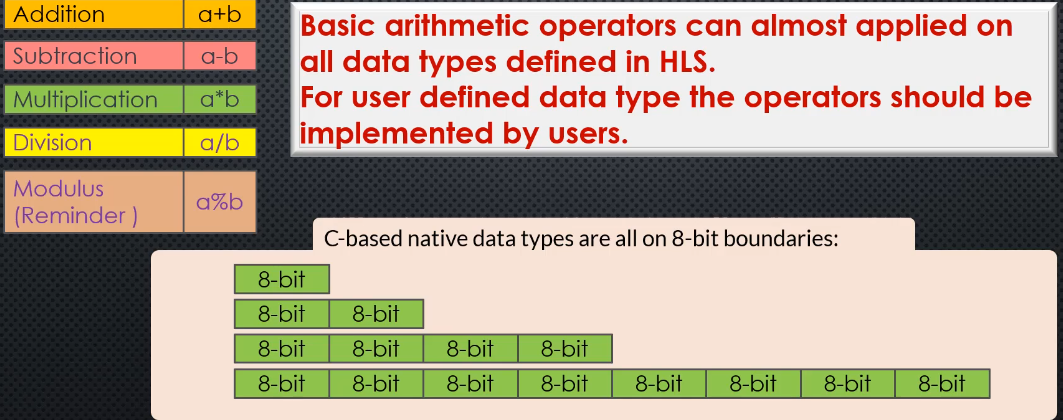
\includegraphics[scale=0.4,frame]{Figures/int_arithmetic/arith_operator}
\caption{Basic Arithmetic Operator}
\label{fig:int_arithmetic:arith_operator}
\end{figure}

These operator can be applied on all native \verb|C| and \verb|C++| data types, and on arbitrary widht data types. Notice that for \verb|C| data types, data type width are multiple of 8 bit, thus operator accuracies are constrained by these boundaries.\\

\todo{operator accruacy} \uti{operator accruacy:}

\begin{itemize}

\item \textit{To see what is that operator accuracy mean, and where it can be applied on. For example:}

	\begin{itemize}
	\item \textit{is there some relation with round off, or truncating error }
	
	\item \textit{the overflow concept also, like the surpassing the capacity of certain range}	
	
	
	\end{itemize}

\end{itemize}

\newpage
Beside from bit width, arithmetic operation can be applied on same data type or different data type, as shown in \autoref{fig:int_arithmetic:arith_operator_data_type}.

\begin{figure}[h]
\centering
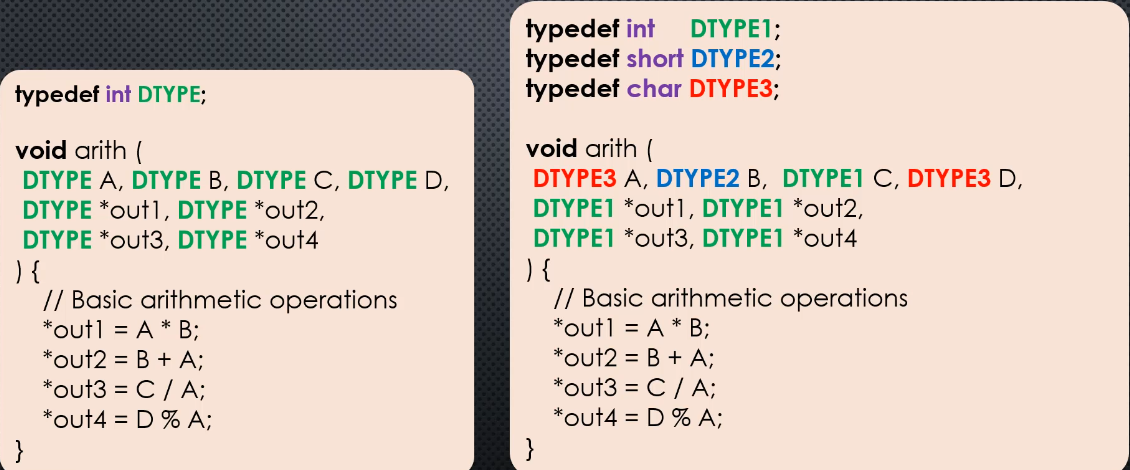
\includegraphics[scale=0.4,frame]{Figures/int_arithmetic/arith_operator_data_type}
\caption{Basic Arithmetic Operator on same or different data type}
\label{fig:int_arithmetic:arith_operator_data_type}
\end{figure}

\begin{itemize}

\item $\mathrm{1}^\mathrm{st}$ example use same data type (\verb|int|) for all argument of the function

\item $\mathrm{2}^\mathrm{nd}$ example uses 3 different data type (\verb|int|,\verb|short| and \verb|char|)

\end{itemize}

\verb|HLS| impelement these operation through \tbi{automatic type casting}.\\

\newpage
\subsection{Circuit types: sequential vs combinational}
\label{sub:circuit_types}

Since in \autoref{part:fundamentals} until now we focus on combinational circuit, we expect that combinational circuit implement arithmetic operation on any data type.

Now let's take a look to what type of operator we have in \verb|HLS| tool as \verb|Vitis|. We have 2 types (shown in \autoref{fig:int_arithmetic:arith_operator_circuit}): combinational and pipeline.

\begin{figure}[h]
\centering
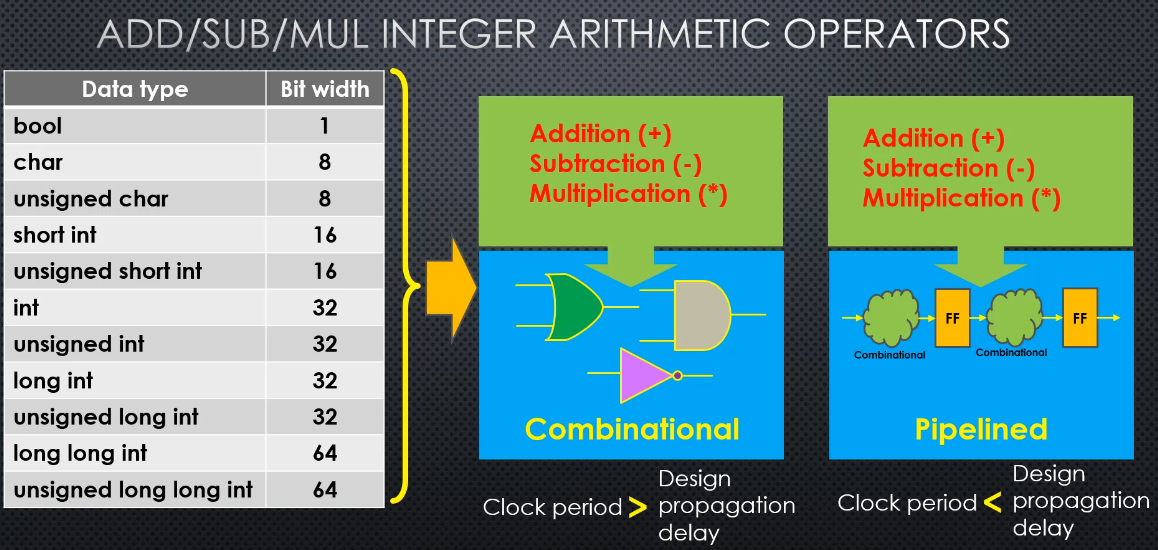
\includegraphics[scale=0.4,frame]{Figures/int_arithmetic/arith_operator_circuit}
\caption{Arithmetic operator and their impelementation}
\label{fig:int_arithmetic:arith_operator_circuit}
\end{figure}

Pipepline circuit uses flip flop (sequential) circuit to minimize $t_p$, and these will be covered in \autoref{part:sequential}.

\todo{Citing Next Part} \textit{Citing Next Part:}

\begin{itemize}

\item \textit{To see how to solve this issue of referecning part of reports}

\end{itemize}

\newpage
There are 2 constraint in choosing between combinational and sequential desing as shown in \autoref{fig:int_arithmetic:circuit_constraint}: the clock period and resources.

\begin{figure}[h]
\centering
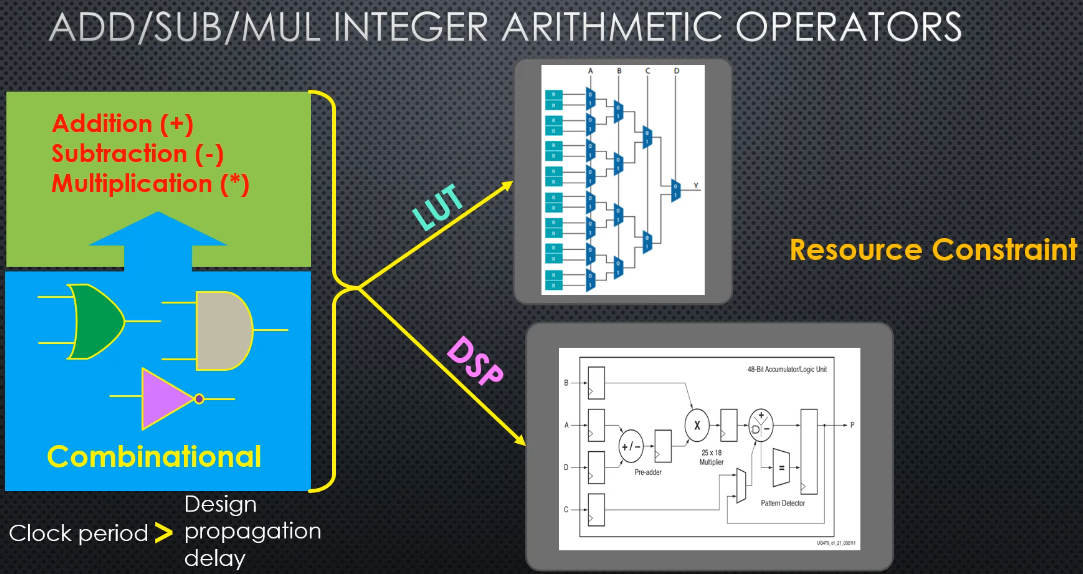
\includegraphics[scale=0.4,frame]{Figures/int_arithmetic/circuit_constraint}
\caption{Circuit Constraint}
\label{fig:int_arithmetic:circuit_constraint}
\end{figure}

\begin{itemize}

\item If the clock period is bigger than the period of arithmetic operations, than combinational circuit is syntehsised

\item Otherwise, sequential circuit is used

\end{itemize}


\newpage
\section{Operator Overloading}

In this section we see how \verb|HLS| uses operator overloaing to apply arithmetic operator on arbitrary precision data type.\\

As a recall, operator overloading is a concept from software programming which adds new implementation based on its argument types. The goal it to use that same operator whith its same standard notation and apply it on the new data type.\\


\autoref{fig:int_arithmetic:op_overloading_hls} shows examples for operator overloading.

\begin{figure}[h]
\centering
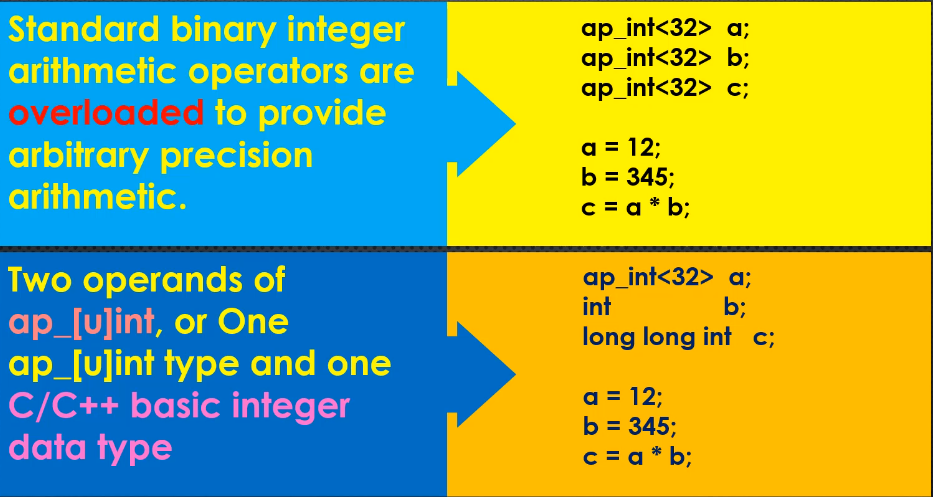
\includegraphics[scale=0.4,frame]{Figures/int_arithmetic/op_overloading_hls}
\caption{Operator Overloading in HLS}
\label{fig:int_arithmetic:op_overloading_hls}
\end{figure} 


\begin{itemize}

\item $\mathrm{1}^\mathrm{st}$ example declare variables of 32 bit width, than use \verb|=| operator to assign some values.

Then there is the usage of \verb|*| operator to do a normal multiplication.

\item $\mathrm{2}^\mathrm{nd}$ example shows how \verb|HLS| uses overloading to accept operand of different type: arbitrary width data type and standard data type from \verb|C| or \verb|C++| language. 

\end{itemize}

\newpage
\autoref{fig:int_arithmetic:op_overloading_function_code} shows example along with functions, where we have the same body but different argument, along with some performance measure after sythesis.

\begin{figure}[h]
\centering
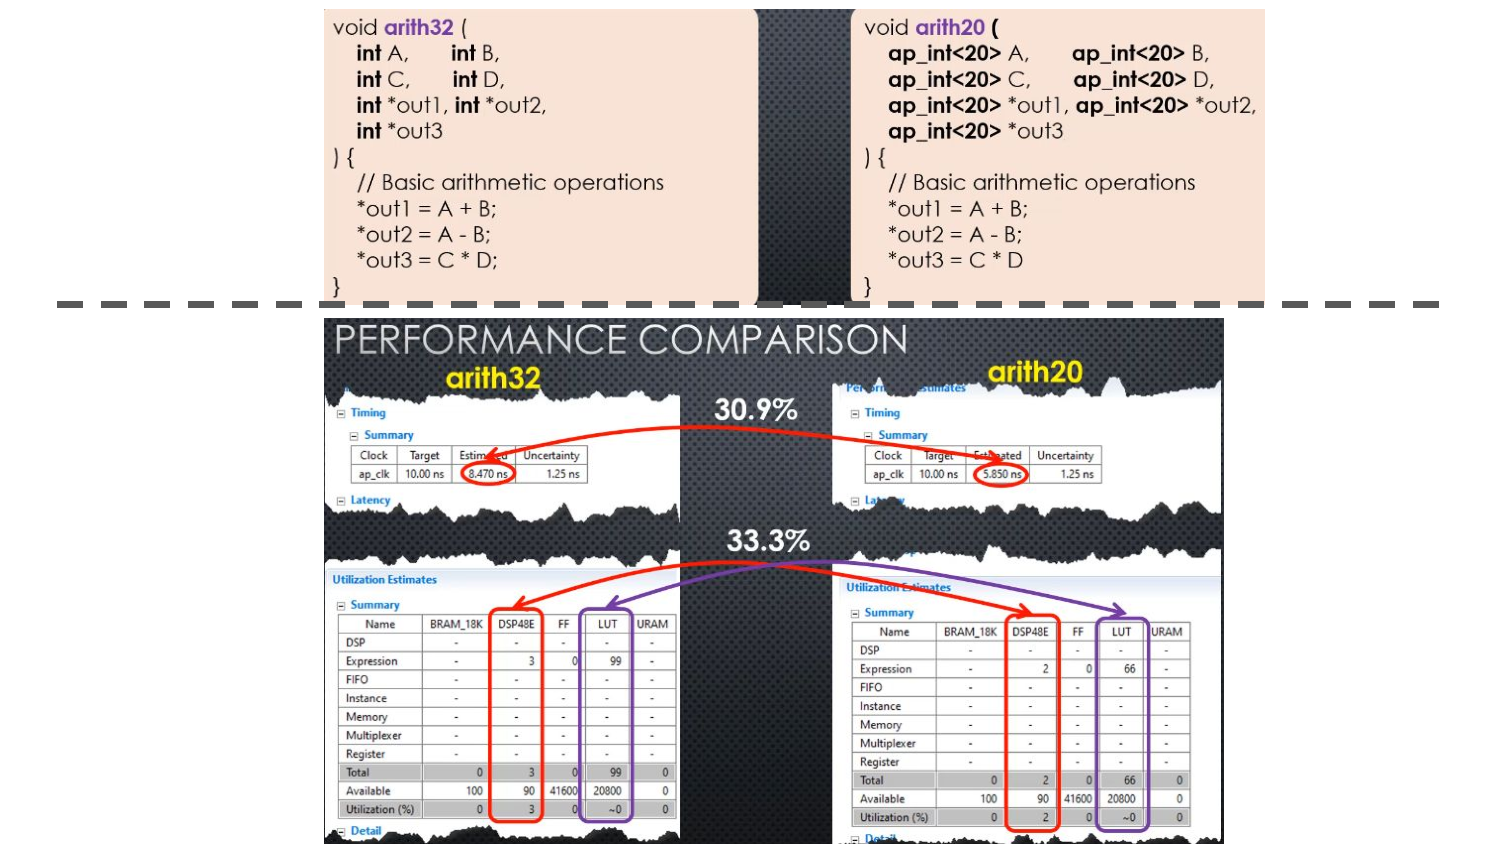
\includegraphics[scale=0.65,frame]{Figures/int_arithmetic/op_overloading_function_code}
\caption{Operator Overloading with functions}
\label{fig:int_arithmetic:op_overloading_function_code}
\end{figure} 

The function with 20 bit data types uses less resources in general.

\subsection{Quiz}

\underline{Given:} Compare the synthesis report of the \verb|HLS| code in \autoref{fig:int_arithmetic:quiz_op_overloading}, for 23 bit datay type and \verb|int| data type.

\begin{figure}[h]
\centering
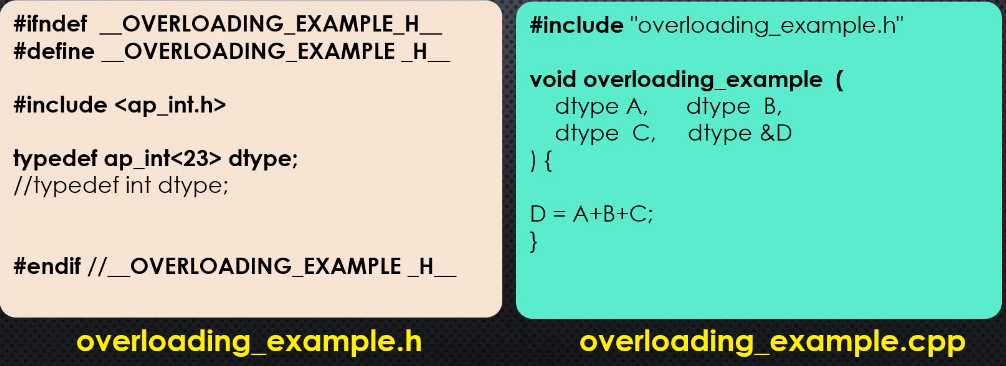
\includegraphics[scale=0.35,frame]{Figures/int_arithmetic/quiz_op_overloading}
\caption{Quiz Operator Overloading}
\label{fig:int_arithmetic:quiz_op_overloading}
\end{figure} 

\newpage
\section{Timing Constraint}


The synthesis of arithmetic expressions into combinational circuit is influenced by the timing constraint of the desing. 


Timing constraint contains 2 elements as shown in \autoref{fig:int_arithmetic:time_constraint}:  

\begin{figure}[h]
\centering
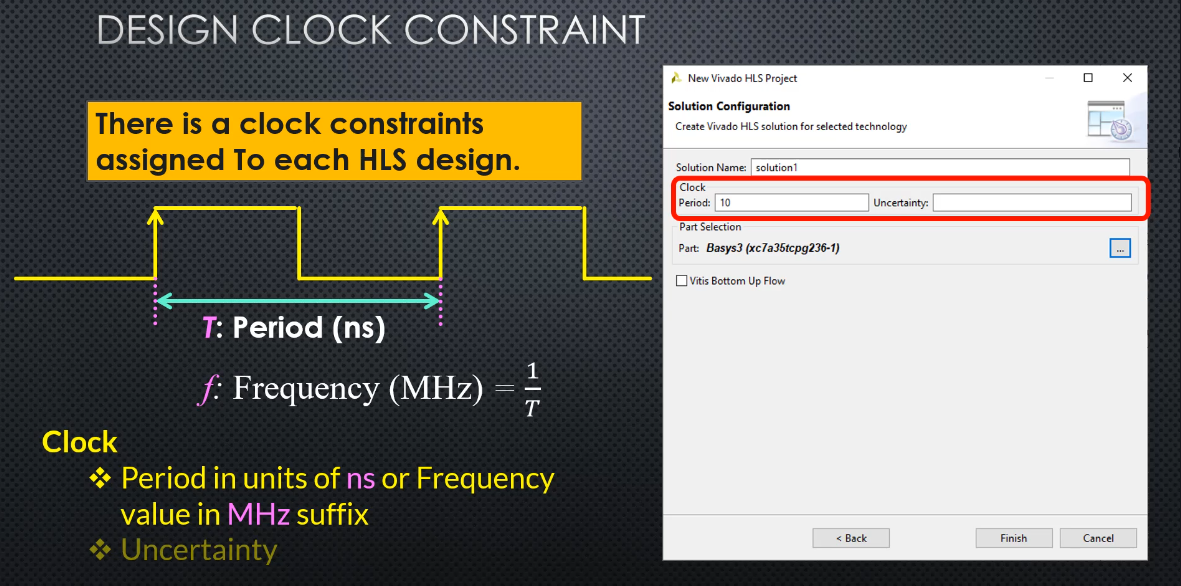
\includegraphics[scale=0.35,frame]{Figures/int_arithmetic/time_constraint}
\caption{Timing constraint: clock period and uncertainty}
\label{fig:int_arithmetic:time_constraint}
\end{figure} 

\begin{itemize}

\item Clock period, which comes in ns for FPGA project or MHz in terms of frequency

\item Uncertainty, which will be covered in part 2 of the course

\end{itemize}


\newpage
Recall from \ref{sub:circuit_types} that the synthesis of digital circuit is related to the clock period and $t_p$. 

\autoref{fig:int_arithmetic:time_constraint_example} presents an example of multiplication function for 2 clock period option: 10 ns (the default one), and the $\mathrm{2}^\mathrm{nd}$ one is chosen to be 5 ns.


\begin{figure}[h]
\centering
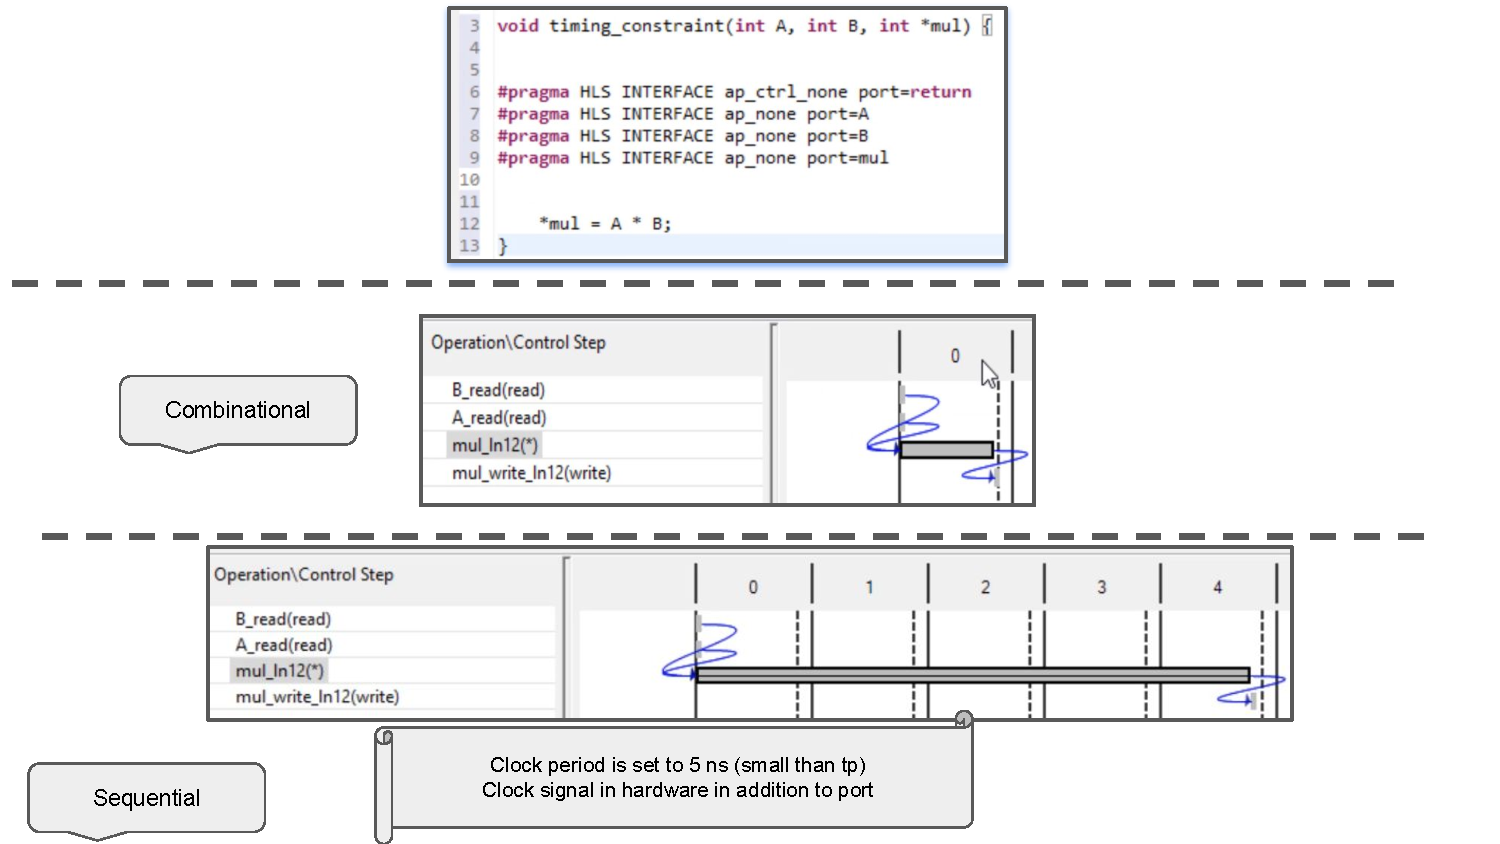
\includegraphics[scale=0.60,frame]{Figures/int_arithmetic/time_constraint_example}
\caption{Timing constraint: clock period and uncertainty}
\label{fig:int_arithmetic:time_constraint_example}
\end{figure}

For the 5 ns, we see that using the analysis perspective that the operation is composed to 5 steps, and it used some memory elements to transfer data between the operations.\\

\todo{Analysis perspective} \uti{Analysis perspective:}

\begin{itemize}

\item \textit{To see how, and train on it, how to use this analysis perspective in Vitis}

\item \textit{Its role in HDL in general, and apply it to HLS}

\end{itemize}


\newpage
\subsection{Quiz}

\underline{Given:} Find a proper value for the clock period to sythesis the code of \autoref{fig:int_arithmetic:quiz_timing_constraint} into a combinational circuit.


\begin{figure}[h]
\centering
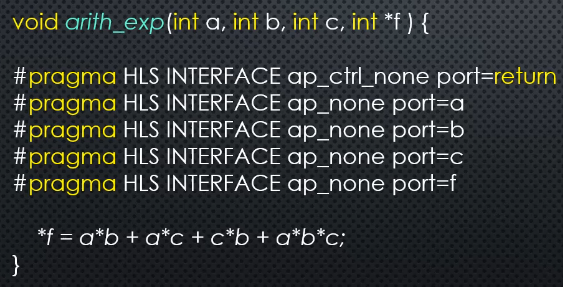
\includegraphics[scale=0.60,frame]{Figures/int_arithmetic/quiz_timing_constraint}
\caption{Quiz timing constraint}
\label{fig:int_arithmetic:quiz_timing_constraint}
\end{figure}

\underline{Solution:} read TimingConstraints-Quiz-Solution.pdf.

\newpage
\section{DSP Resources}

To implement arithmetic expressions, FPGA comes traditionally with LUT, which works under simple scenarios. But for applications wich requires more computaitonal demands, FPGA vendors introduces DSP blocks, wihch have high performance for complex computation task.

\begin{figure}[h]
\centering
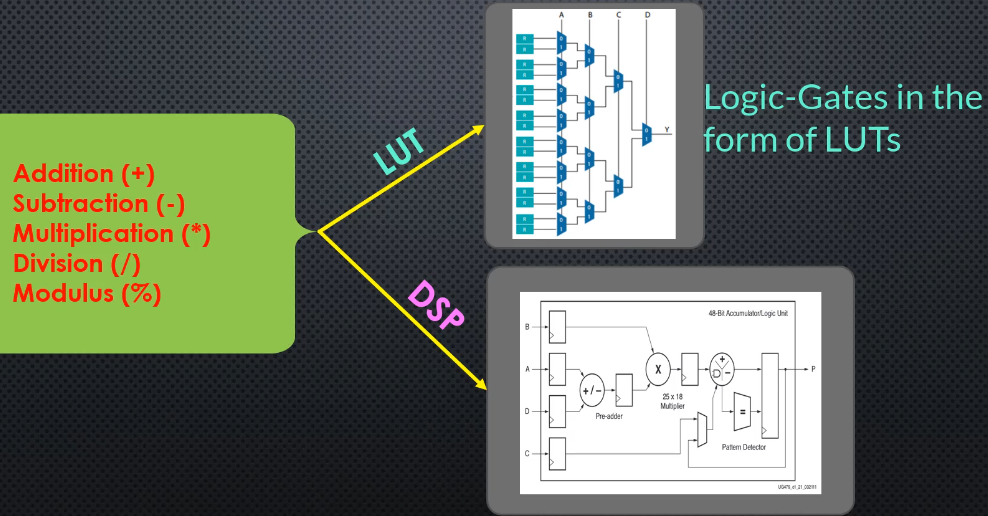
\includegraphics[scale=0.40,frame]{Figures/int_arithmetic/arithmetic_resources}
\caption{Arithmetic Resources}
\label{fig:int_arithmetic:arithmetic_resources}
\end{figure}

A typical DSP block receives a couple of inputs and then passes them through a set of pre-designed reconfigurable
addition and multiplication modules. \autoref{fig:int_arithmetic:DSP48_block} shows a DSP48 block which is used in \verb|Basys3| board.


\begin{figure}[h]
\centering
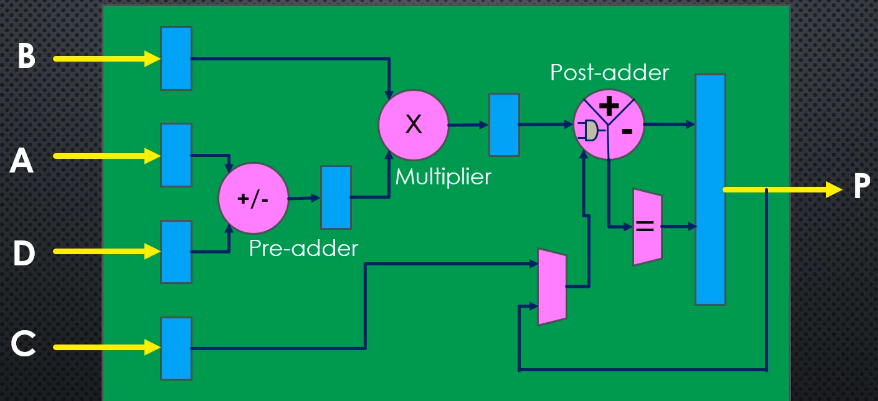
\includegraphics[scale=0.40,frame]{Figures/int_arithmetic/DSP48_block}
\caption{DSP Block}
\label{fig:int_arithmetic:DSP48_block}
\end{figure}

\verb|HLS| tools usually automate all computation steps, but havving some familiarity with mechanism inside the DSP block help us to guide us for the synthesis process to generate high performance RTL descirption.\\

\todo{DSP block and RTL description} \uti{DSP block and RTL description:}

\begin{itemize}

\item \textit{To see later when starting the VHDL course, the role of FPGA block in general, like the LUT, DSP,memories,$\cdots$}

	\begin{itemize}
	\item \textit{Try to see some resources like papers, github,$\cdots$ to see how to simulations and study to optmize these resources}
	\end{itemize}

\end{itemize}

\subsection{DSP description}

\begin{itemize}

\item At the heart of the DSP, there is a multiplier that accepts a 25 bit and an 18 bit two's complement
inputs and generates a 43 bit two's complement result.

\item This multiplier receives one of its inputs via a pre adder module and gives its output to a post adder
module.

\item There are also other paths in a DSP to provide enough data path to implement different mathematical
and logical expressions.

\item Most data paths inside the DSP can be registered in flip flops.

\item In addition, the multiplier and additions inside the DSP can be implemented by a single stage combinational circuit or a multi-stage pipeline structure.

\end{itemize}

\todo{DSP description} \uti{DSP description:}

\begin{itemize}

\item \textit{There are to much theory, to see later some other resources to understand them}

\end{itemize}

\newpage
\subsection{DSP Example}

Let's see now how a DSP can be reconfigured using the 2 cases of \autoref{eq:dsp_example}.

\begin{equation}
\begin{array}{rcl}
f \, &=& \, A \, \star \, B \\
f \, &=& \, (A \, + \, B) \, \star \, D 
\end{array}
\label{eq:dsp_example}
\end{equation}

\autoref{fig:int_arithmetic:dsp_example} shows their graph representation along with the data path in for each DSP block.

\begin{figure}[h]
\centering
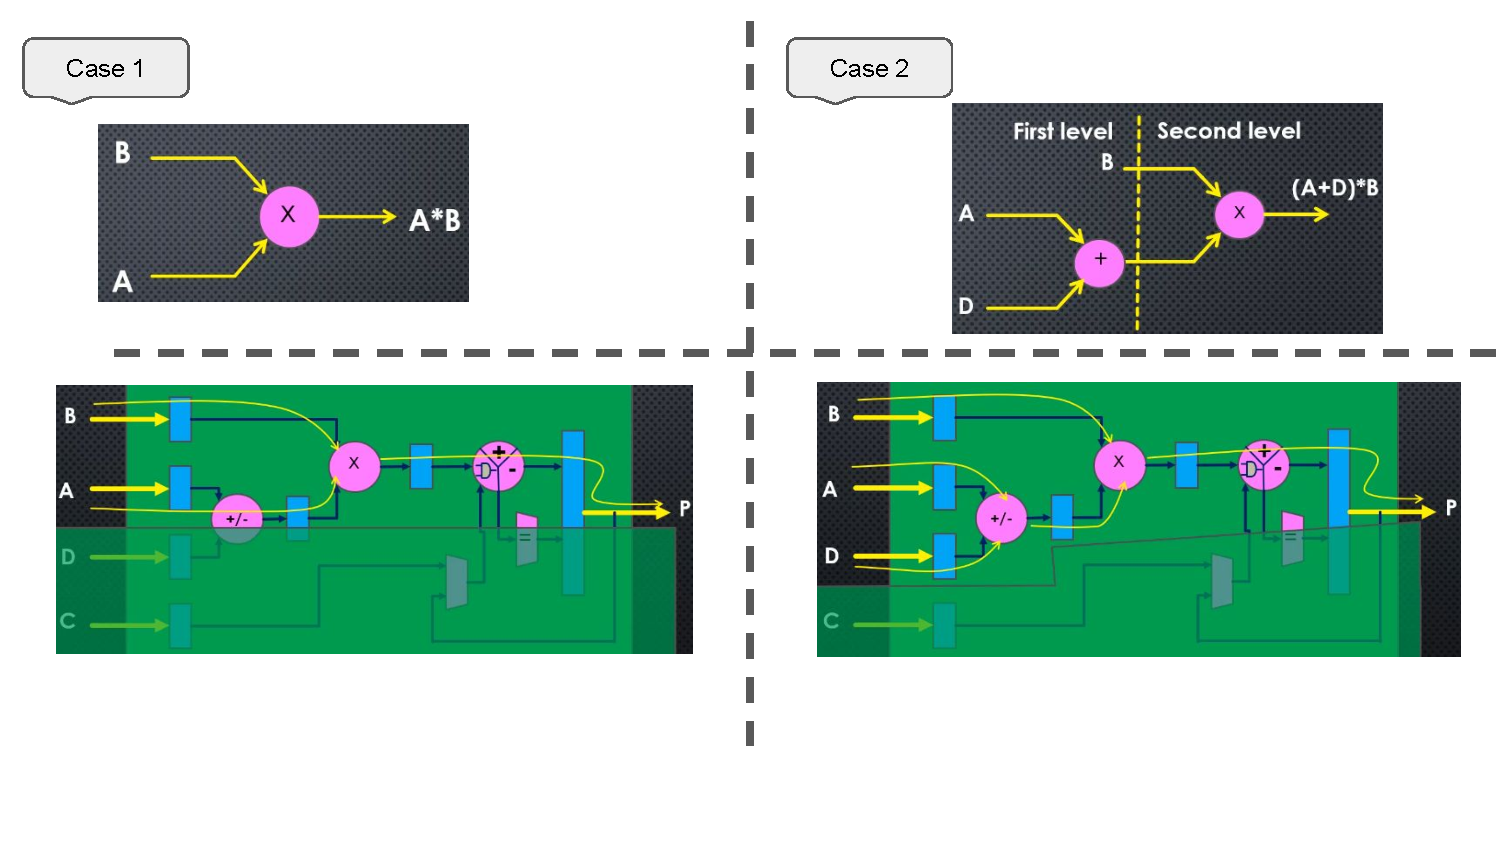
\includegraphics[scale=0.55,frame]{Figures/int_arithmetic/dsp_example}
\caption{DSP Example}
\label{fig:int_arithmetic:dsp_example}
\end{figure}


\begin{itemize}

\item \underline{Case 1:} $B$ input feeds the multiplier directly.

$A$ bypasse the adder and it is connected to the multiplier

Finally, the multipler result gets to the output by avoinding all the operators along the path 

\item \underline{Case 2:} Same principle as in case 1, but this epxression has 2 level in its graph

\end{itemize}


\todo{DSP Examples} \uti{DSP Examples:}

\begin{itemize}

\item \textit{Is there any relation between the graph and the DSP ? maybe concerning its path}

	\begin{itemize}
	\item \textit{To be seen later}
	\end{itemize}

\item \textit{Can we implement epxression with more than 4 inputs to this DSP48 block?}

	\begin{itemize}
	\item \textit{Maybe need more complex DSP}
	
	\item \textit{Or this DSP48 can reconfigure and evolve to handle more complex expresssions}
	
	\item \textit{To be seen later}
	\end{itemize}

\end{itemize}


\newpage
\section{Resource Selection}

We saw that the implementation of arithmetic and logic expression can be done via 2 resources: LUT and DSP blocks. In this section we see how to guide the synthesis tools to choose between these 2 resources.\\


In order to implement \verb|C/C++| code into hardware resources, \verb|Vitis| perform 2 task: elaboration and mapping.

\begin{figure}[h]
\centering
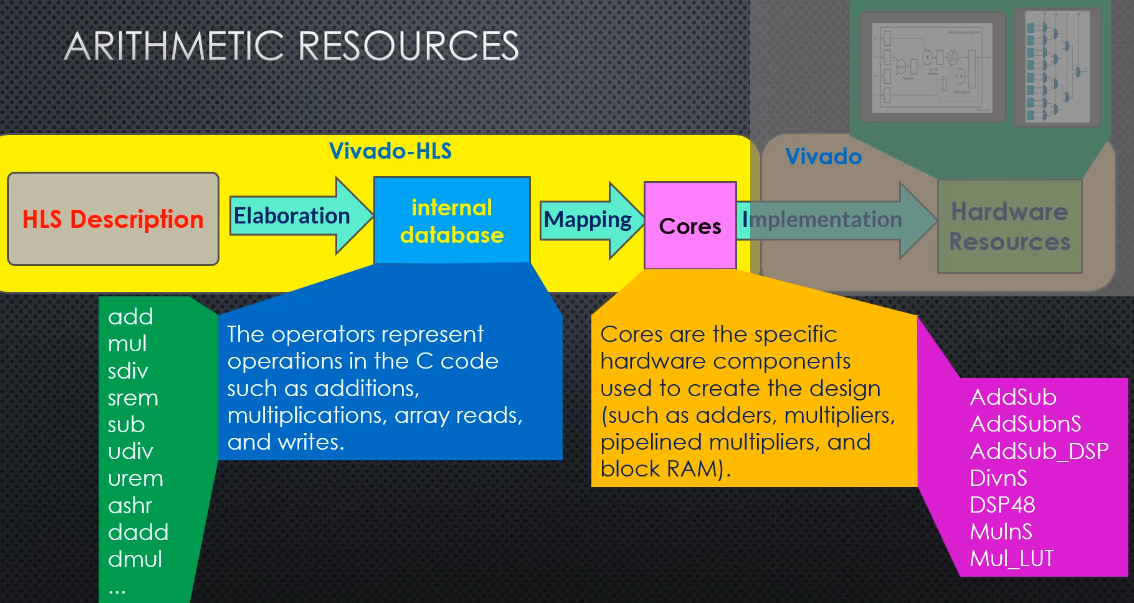
\includegraphics[scale=0.40,frame]{Figures/int_arithmetic/vitis_elab_mapp}
\caption{Elaboration and Mapping}
\label{fig:int_arithmetic:vitis_elab_mapp}
\end{figure}

\begin{itemize}

\item Elaboration: is where the \verb|C| code is transformed into a database containing different elements. 

Each element of this database contains \verb|C| operatiosn such as addition, multiplication,array read and write,$\cdots$

\item Mapping: this task maps the operator (saved in elaboration step) onto a set of \textit{cores} which implement hardware resources

	\begin{itemize}
	\item Example of cores \verb|AddSub|,$\cdots$ (list is shown in \autoref{fig:int_arithmetic:cores_example}).
	\end{itemize}

\end{itemize}

\newpage
\begin{figure}[h]
\centering
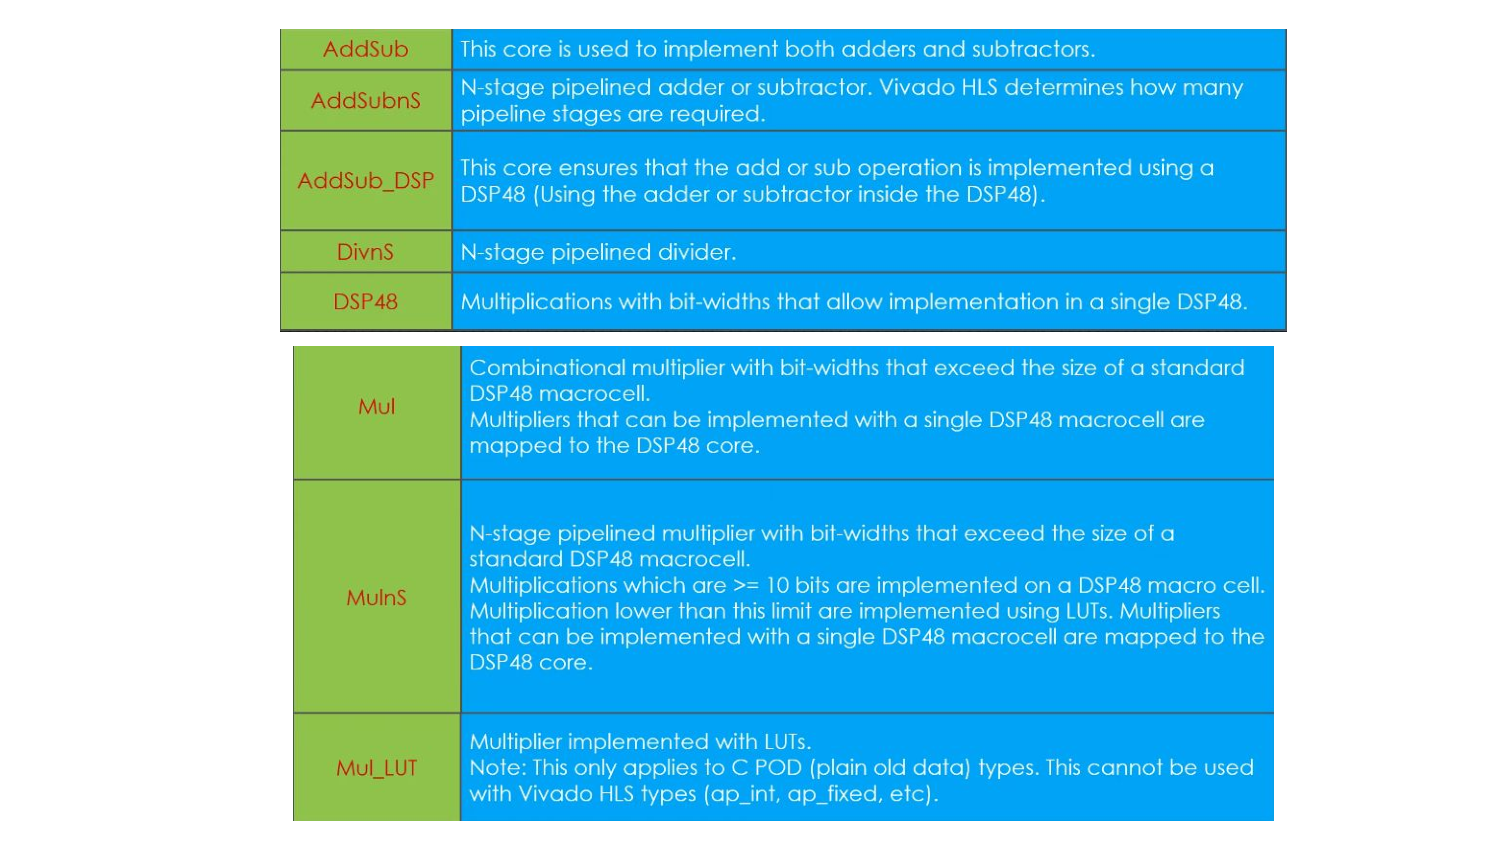
\includegraphics[scale=0.60,frame]{Figures/int_arithmetic/cores_example}
\caption{Hardware Cores Example}
\label{fig:int_arithmetic:cores_example}
\end{figure}


\subsection{Examples}

In \verb|HLS|, there are 2 pragma directive to use these core resources on operators: \verb|ALLOCATION| and \verb|RESOURCE|. 

\begin{figure}[h]
\centering
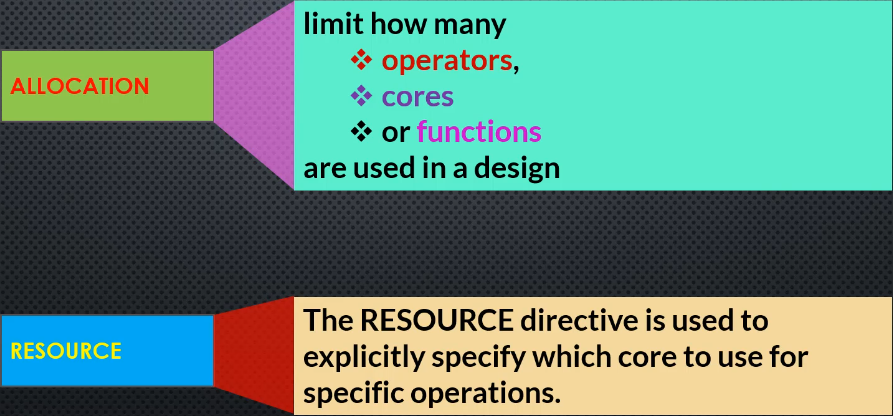
\includegraphics[scale=0.40,frame]{Figures/int_arithmetic/resrc_directive}
\caption{Resource directives}
\label{fig:int_arithmetic:resrc_directive}
\end{figure}

Let's take several examples to see how to use these directive.

\newpage
$\mathrm{1}^\mathrm{st}$ example is shown in \autoref{fig:int_arithmetic:resrc_ex1}, where \verb|f| is the output of the operator.

\begin{figure}[h]
\centering
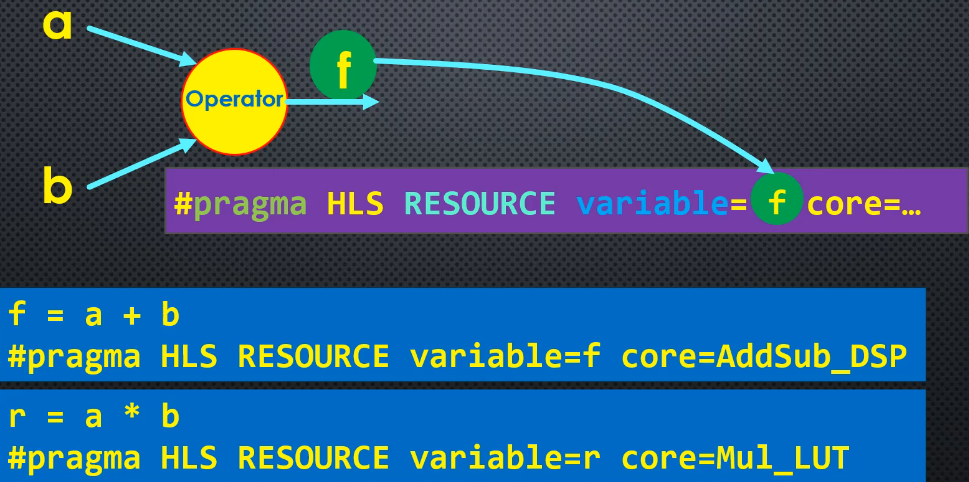
\includegraphics[scale=0.40,frame]{Figures/int_arithmetic/resrc_ex1}
\caption{Example 1 of resource usage: DSP and LUT}
\label{fig:int_arithmetic:resrc_ex1}
\end{figure}

\begin{itemize}

\item using \verb|#pragma HLS RESOURCE variable=f core=...|,  \verb|HLS| tool know which resource to use for the synthesis for the \verb|f| expression

\item 2 examples are used for the operator: \verb|+| and \verb|*|

	\begin{itemize}
	
	\item The addition is performed using DSP block through \verb|core=AddSub_DSP|

	\item The multiplication is perfomed using LUT through \verb|core=Mul_LUT|
	
	\end{itemize}

\end{itemize}

\autoref{fig:int_arithmetic:resrc_ex2} presents an expression with multiple operator. 

\begin{figure}[h]
\centering
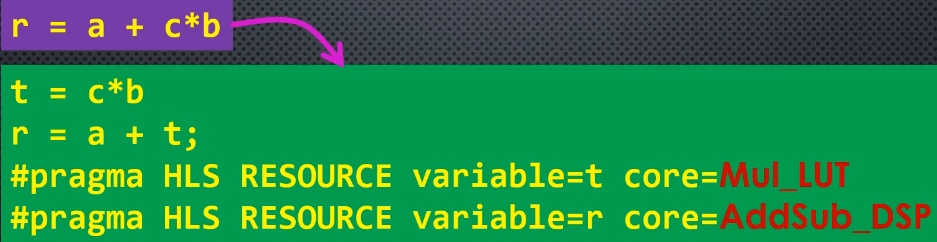
\includegraphics[scale=0.40,frame]{Figures/int_arithmetic/resrc_ex2}
\caption{Expression with multiple operators}
\label{fig:int_arithmetic:resrc_ex2}
\end{figure}

The key it to break down the expression into a set of expression of 1 opertors, then use the \verb|#pragma| on each expression.

\todo{$\mathrm{3}^\mathrm{rd}$ example} \uti{$\mathrm{3}^\mathrm{rd}$ example:}

\begin{itemize}

\item \textit{source: section 12, video 12, from time 4:22}

\item \textit{it is about implementing a complex arithmetic expression in Vitis, using LUT and DSP}

\item \textit{It uses the analysis perspective and change the clock rate}

	\begin{itemize}
	\item \textit{I didn't understand all the details yet, to redo when doing a complete revision about the $\mathrm{1}^\mathrm{st}$ part, and digital logic part also}
	\end{itemize}

\end{itemize}


\newpage
\section{Integer Division and Modulus}

Integer division and modulus need special attention when  when it comes to synthesizing them into combinational circuits.\\

As a reminder, integer division returns the quotient and modulus returns the reminder, as shown in the example of 
\autoref{fig:int_arithmetic:div_mod}.

\begin{figure}[h]
\centering
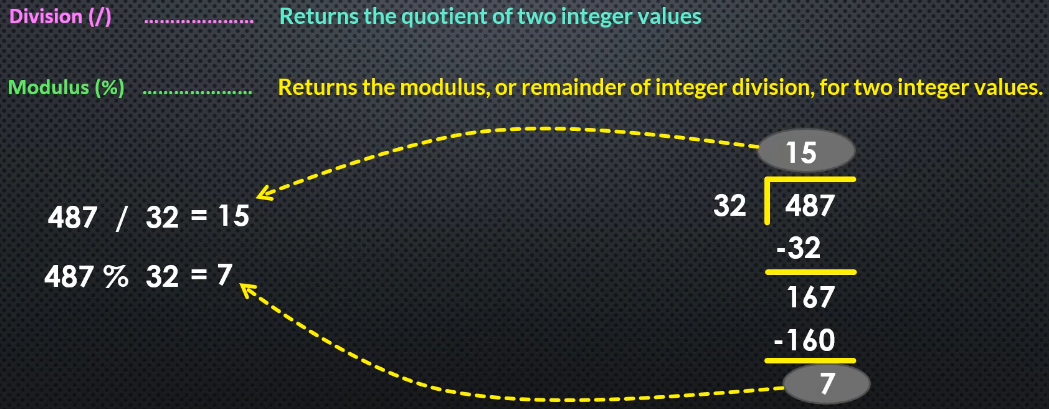
\includegraphics[scale=0.40,frame]{Figures/int_arithmetic/div_mod}
\caption{Division and Moudulus}
\label{fig:int_arithmetic:div_mod}
\end{figure}

Let's see different cases for \verb|/| and \verb|%| operations.

The pragma used: \verb|#pragma HLS RESOURCE variable=r core=Divns|.\\

\underline{Different cases:}

\begin{enumerate}

\item Division: \verb|r = a/n;|

	\begin{itemize}
	\item pipeline by default (with or no \verb|pragma| used)
	
	\item if \verb|const int n;|, then it synthesis combinational if clock period $> \, t_p$
	\end{itemize}

\item Modulus: \verb|r = a%n|

	\begin{itemize}
	\item pipeline also by default
	
	\item if \verb|const int n|, we can use the equivalent expression \verb|r = a - n*(a/n)|
	\end{itemize}

\end{enumerate}


\todo{division and moudlus demo} \uti{division and moudlus demo:}

\begin{itemize}

\item  \textit{source: section 12, video 103, t = 3:05}

\item \textit{Also various demo using Vitis, but to do later when reviweing the digital desing part, computer arithmetic,$\cdots$}

\item \textit{To see if his explanation and notes has some benifits or not, or just some theory applied}

\end{itemize}

\section{Quiz}

See the file IntegerArithmetic-Exercise-Solution in \verb|Other_Resources| directory.
